%!tikz editor 1.0
%!tikz source begin
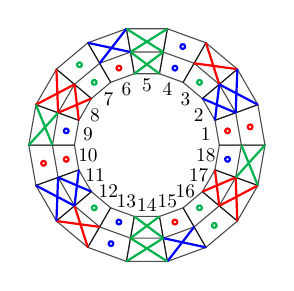
\begin{tikzpicture}[scale=.4,every node/.style={scale=.7}]

	%% Settings
	\pgfmathsetmacro{\Nutzahl}{18}
	\pgfmathsetmacro{\Spulenweite}{2}	

	\pgfmathsetmacro{\rNummerInnen}{1.9}
	\pgfmathsetmacro{\rInnen}{2.3}
	\pgfmathsetmacro{\rMitte}{3}
	\pgfmathsetmacro{\rAussen}{3.75}
	\pgfmathsetmacro{\rAngleOffset}{360/\Nutzahl/2}
	
	%% Background Pattern
	\foreach \i in {1,2,...,\Nutzahl}
	{	
		\draw [opacity=0.7] [rotate=(\i-1)*(360/\Nutzahl)]
			(0:\rMitte) -- (0:\rAussen) -- (360/\Nutzahl:\rAussen) -- (360/\Nutzahl:\rMitte) -- (0:\rMitte)
			(0:\rInnen) -- (0:\rMitte) -- (360/\Nutzahl:\rMitte) -- (360/\Nutzahl:\rInnen) -- (0:\rInnen);
		\node at (\i*360/\Nutzahl-\rAngleOffset:\rNummerInnen) {\i};		
	}

	%% Inner
	% red
	\foreach \i in {1,6,10,15}
	{	
		\draw [rotate=(\i-1)*(360/\Nutzahl), thick, color=red]
			(180/\Nutzahl:2.6) circle (0.075);
		\draw [rotate=(\i-1+\Spulenweite)*(360/\Nutzahl), thick, color=red]
			(0:\rMitte) -- (360/\Nutzahl:\rAussen) (0:\rAussen) -- (360/\Nutzahl:\rMitte);
	}
	\foreach \i in {8,17}
	{	
		\draw [rotate=(\i-1)*(360/\Nutzahl), thick, color=red]
			(0:\rInnen) -- (360/\Nutzahl:\rMitte) (0:\rMitte) -- (360/\Nutzahl:\rInnen);
		\draw [rotate=(\i-1+\Spulenweite)*(360/\Nutzahl), thick, color=red]
			(180/\Nutzahl:3.33) circle (0.075);
	}
	
	% blue
	\foreach \i in {4,9,13,18}
	{	
		\draw [rotate=(\i-1)*(360/\Nutzahl), thick, color=blue]
			(180/\Nutzahl:2.6) circle (0.075);
		\draw [rotate=(\i-1+\Spulenweite)*(360/\Nutzahl), thick, color=blue]
			(0:\rMitte) -- (360/\Nutzahl:\rAussen) (0:\rAussen) -- (360/\Nutzahl:\rMitte);
	}
	\foreach \i in {2,11}
	{	
		\draw [rotate=(\i-1)*(360/\Nutzahl), thick, color=blue]
			(0:\rInnen) -- (360/\Nutzahl:\rMitte) (0:\rMitte) -- (360/\Nutzahl:\rInnen);
		\draw [rotate=(\i-1+\Spulenweite)*(360/\Nutzahl), thick, color=blue]
			(180/\Nutzahl:3.33) circle (0.075);
	}
	
	% green
	\foreach \i in {3,7,12,16}
	{	
		\draw [rotate=(\i-1)*(360/\Nutzahl), thick, color=green!70!blue]
			(180/\Nutzahl:2.6) circle (0.075);
		\draw [rotate=(\i-1+\Spulenweite)*(360/\Nutzahl), thick, color=green!70!blue]
			(0:\rMitte) -- (360/\Nutzahl:\rAussen) (0:\rAussen) -- (360/\Nutzahl:\rMitte);
	}
	\foreach \i in {5,14}
	{	
		\draw [rotate=(\i-1)*(360/\Nutzahl), thick, color=green!70!blue]
			(0:\rInnen) -- (360/\Nutzahl:\rMitte) (0:\rMitte) -- (360/\Nutzahl:\rInnen);
		\draw [rotate=(\i-1+\Spulenweite)*(360/\Nutzahl), thick, color=green!70!blue]
			(180/\Nutzahl:3.33) circle (0.075);
	}
	
\end{tikzpicture}
%!tikz source end
